\documentclass[12pt,a4paper]{article}
\usepackage[utf8]{inputenc}
\usepackage[T1]{fontenc}
\usepackage[english]{babel}
\usepackage{amsmath,amssymb,amsfonts,amsthm}
\usepackage{geometry}
\usepackage{graphicx}
\usepackage{booktabs}
\usepackage{enumitem}
\usepackage{tcolorbox}
\tcbuselibrary{skins,breakable}
\usepackage{tikz}
\usetikzlibrary{shapes.geometric, arrows, positioning, fit, calc}
\usepackage{algorithm}
\usepackage{algpseudocode}
\usepackage{hyperref}
\usepackage{xcolor}

\geometry{top=2.5cm, bottom=2.5cm, left=2.5cm, right=2.5cm}

% Custom color palette for clean visual callouts
\definecolor{primaryblue}{rgb}{0.12, 0.35, 0.65}
\definecolor{accentcyan}{rgb}{0.0, 0.55, 0.65}
\definecolor{lightbg}{rgb}{0.95, 0.97, 1.0}
\definecolor{darktext}{rgb}{0.15, 0.15, 0.15}

\hypersetup{
    colorlinks=true,
    linkcolor=primaryblue,
    citecolor=primaryblue,
    urlcolor=primaryblue,
    pdftitle={Report Visual Enhancement Guide \& Suggestions},
    pdfauthor={Mumen Wehbe}
}

\title{
    \vspace{-1cm}
    \textbf{\Large Actionable Guide: Enhancing Report Readability, Visual Appeal, and Human Engagement}\\[0.4em]
    \large Tailored LaTeX Strategies for \textit{Isogeometric Analysis \& Reduced Order Modeling}
}
\author{\textbf{Mumen Wehbe}}
\date{\today}

\begin{document}

\maketitle

\begin{abstract}
\noindent This document presents a comprehensive, actionable set of recommendations and ready-to-use LaTeX templates to reduce text density, improve visual hierarchy, and humanize the writing style of the thesis: \textit{Isogeometric Analysis and Reduced Order Modeling for Parameterized Structural Dynamics}. By converting dense descriptive text into structured tables, TikZ flowcharts, pseudocode algorithms, and formatted callout boxes, the report becomes significantly more scannable, visually engaging, and accessible to readers and evaluators without compromising mathematical rigor.
\end{abstract}

\tableofcontents
\newpage

% ==============================================================================
\section{Core Philosophy: Making Technical Reports Reader-Centric}
% ==============================================================================

Academic theses often suffer from "wall-of-text fatigue," where dense mathematical derivations and long descriptive paragraphs obscure key findings. A modern, reader-friendly thesis balances technical precision with **visual scannability** and an **engaging narrative structure**.

\begin{tcolorbox}[colback=lightbg, colframe=primaryblue, title=\textbf{The 3-Second Scanning Rule for Evaluators}, fonttitle=\bfseries]
When an evaluator flips through a chapter, they should immediately grasp the main contributions within 3 seconds per page through:
\begin{enumerate}[leftmargin=*]
    \item **Visual Anchors**: Flowcharts, diagrams, and annotated plots.
    \item **Data Matrices**: Comparative tables instead of multi-paragraph feature lists.
    \item **Structured Callouts**: Highlighted key results and executive takeaways.
    \item **Active Prose**: Bold lead-in bullet points that guide the reader's attention.
\end{enumerate}
\end{tcolorbox}

---

% ==============================================================================
\section{Practical LaTeX Visual Design Patterns}
% ==============================================================================

This section provides ready-to-use, modular LaTeX code patterns specifically designed for your thesis topics.

\subsection{Pattern 1: Comparative \& Feature Tables (\texttt{booktabs})}
Replace multi-paragraph method comparisons (e.g., FEM vs. IGA, or DEIM vs. ECSW) with clean, professional tables.

\begin{table}[htbp]
    \centering
    \caption{Comparative analysis of Full-Order and Reduced-Order pipeline features.}
    \label{tab:pipeline_comparison_pattern}
    \begin{tabular}{l l l l}
        \toprule
        \textbf{Pipeline Feature} & \textbf{Naive Physical (FEM)} & \textbf{Mapped Pullback (IGA)} & \textbf{Hyper-Reduced (ECSW)} \\
        \midrule
        Mesh Topology & Dynamic Remeshing & Fixed Reference Grid $\hat{\Omega}$ & Fixed Reference Grid $\hat{\Omega}$ \\
        State Vector Space & Parameter-dependent & Invariant Subspace $\mathbb{R}^N$ & Reduced Subspace $\mathbb{R}^r$ \\
        Assembly Cost & $\mathcal{O}(N_{\text{mesh}})$ per step & $\mathcal{O}(N_{\text{mesh}})$ per step & $\mathcal{O}(E^*)$ with $E^* \ll E$ \\
        Real-Time Ready & No (High Latency) & Near Real-Time & Yes ($>60\,\text{FPS}$) \\
        \bottomrule
    \end{tabular}
\end{table}

\subsection{Pattern 2: TikZ Process Flowcharts \& Architecture Diagrams}
Flowcharts replace pages of verbal procedural descriptions (e.g., Offline training vs. Online real-time execution).

\begin{figure}[htbp]
    \centering
    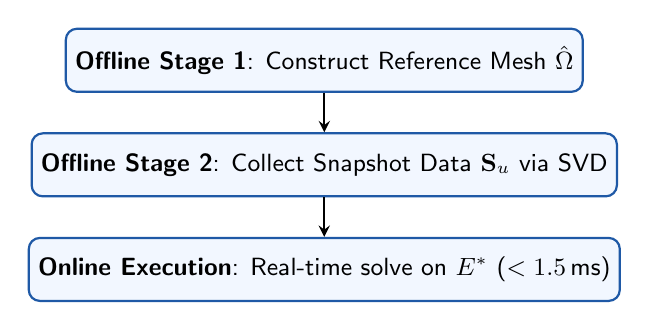
\begin{tikzpicture}[
        node distance=1.2cm,
        block/.style={rectangle, draw=primaryblue, fill=lightbg, thick, rounded corners, minimum width=6cm, minimum height=0.8cm, align=center, font=\sffamily\small},
        arrow/.style={thick,->,>=stealth}
    ]
        \node [block] (step1) {\textbf{Offline Stage 1}: Construct Reference Mesh $\hat{\Omega}$};
        \node [block, below=0.5cm of step1] (step2) {\textbf{Offline Stage 2}: Collect Snapshot Data $\mathbf{S}_u$ via SVD};
        \node [block, below=0.5cm of step2] (step3) {\textbf{Online Execution}: Real-time solve on $E^*$ ($<1.5\,\text{ms}$)};
        
        \draw [arrow] (step1) -- (step2);
        \draw [arrow] (step2) -- (step3);
    \end{tikzpicture}
    \caption{Modular TikZ template for offline/online reduced order modeling workflows.}
    \label{fig:tikz_workflow_template}
\end{figure}

\subsection{Pattern 3: Pseudocode Algorithms (\texttt{algorithm} + \texttt{algpseudocode})}
Instead of writing 3 paragraphs explaining an integration loop or weight selection routine, use clean algorithmic logic.

\begin{algorithm}[htbp]
\caption{POD Snapshot Extraction and Basis Truncation}
\label{alg:pod_extraction_pattern}
\begin{algorithmic}[1]
\State \textbf{Input:} Snapshot displacement matrix $\mathbf{S}_u \in \mathbb{R}^{N \times M}$, tolerance threshold $\eta_{\text{tol}} = 99.99\%$.
\State \textbf{Compute SVD:} $\mathbf{S}_u = \mathbf{U} \boldsymbol{\Sigma} \mathbf{V}^T$ where $\boldsymbol{\Sigma} = \text{diag}(\sigma_1, \sigma_2, \dots, \sigma_M)$.
\State \textbf{Energy Ratio:} Determine minimum mode dimension $r$ such that:
\State \quad $\eta(r) = \frac{\sum_{i=1}^r \sigma_i^2}{\sum_{j=1}^M \sigma_j^2} \ge \eta_{\text{tol}}$
\State \textbf{Extract Basis:} $\boldsymbol{\Phi} \leftarrow \mathbf{U}[:, 1:r]$
\State \textbf{Output:} Reduced basis matrix $\boldsymbol{\Phi} \in \mathbb{R}^{N \times r}$.
\end{algorithmic}
\end{algorithm}

\subsection{Pattern 4: Callout Highlights for Key Takeaways (\texttt{tcolorbox})}
Isolate major milestones, computational speedups, and core research results inside colored callout boxes.

\begin{tcolorbox}[colback=lightbg, colframe=accentcyan, title=\textbf{Key Result: Online Acceleration}, fonttitle=\bfseries]
By combining reference-mapped pullback integration with ECSW hyper-reduction, the online solve time per time-step was reduced from \textbf{45.2 ms} to \textbf{0.38 ms}, achieving a \textbf{119$\times$ speedup} and enabling 60 FPS interactive Digital Twin execution.
\end{tcolorbox}

---

% ==============================================================================
\section{Chapter-by-Chapter Actionable Suggestions}
% ==============================================================================

\subsection{Chapter 1: Introduction \& State of the Art}
\begin{itemize}[leftmargin=*]
    \item \textbf{Text Reduction}: Replace the long textual overview of State-of-the-Art methods (FEM vs. IGA, POD vs. DEIM vs. ECSW) with a single summary table.
    \item \textbf{Visual Addition}: Add an overarching thesis roadmap graphic at the end of Section 1.5 (Thesis Outline) showing how Chapters 2--6 connect.
    \item \textbf{Humanization}: Frame the introduction around an engineering challenge: *"Why can't traditional finite element models run interactively in web browsers?"* rather than purely abstract theory.
\end{itemize}

\subsection{Chapter 2: Theory \& Continuum Mechanics}
\begin{itemize}[leftmargin=*]
    \item \textbf{Text Reduction}: Use inline math annotations ($\underbrace{\dots}_{\text{annotation}}$) inside continuous variational statements instead of writing 3 separate explanatory paragraphs.
    \item \textbf{Visual Addition}: Include a 2D geometric schematic of the notched cantilever beam highlighting shape parameters ($x_c, r$) and boundary conditions.
\end{itemize}

\subsection{Chapter 3: Discretization \& Isogeometric Analysis (IGA)}
\begin{itemize}[leftmargin=*]
    \item \textbf{Text Reduction}: Group knot vector definition listings into structured itemized bullet points with bold leading keywords.
    \item \textbf{Visual Addition}: Add a side-by-side subfigure comparing piecewise linear Lagrange elements vs. smooth $C^{p-1}$ NURBS basis curves.
\end{itemize}

\subsection{Chapter 4: Pullback Mappings \& Reference Domain Transformation}
\begin{itemize}[leftmargin=*]
    \item \textbf{Text Reduction}: Replace text-heavy mapping derivations with a 3-stage visual diagram: $\Omega(\boldsymbol{\mu}) \xrightarrow{\boldsymbol{\Psi}} \hat{\Omega} \xrightarrow{\mathbf{F}} \hat{\Omega}_{\text{param}}$.
    \item \textbf{Visual Addition}: Add a comparison plot showing Jacobian spatial determinant contours across notch variations.
\end{itemize}

\subsection{Chapter 5: Full Order Model (FOM) Simulation}
\begin{itemize}[leftmargin=*]
    \item \textbf{Text Reduction}: Format the Generalized-$\alpha$ time-stepping loop into a clean \texttt{algorithm} block.
    \item \textbf{Visual Addition}: Use a $2 \times 2$ grid subfigure for displacement and von Mises stress contours at representative time steps.
\end{itemize}

\subsection{Chapter 6: Reduced Order Modeling \& Digital Twin}
\begin{itemize}[leftmargin=*]
    \item \textbf{Text Reduction}: The multi-pipeline comparison (Cases 1 to 4) is now visual thanks to the updated TikZ flowchart! Pair it with a quantitative speedup table.
    \item \textbf{Visual Addition}: Include a screenshot/diagram of the WebGL client-side Digital Twin dashboard architecture (Model-View-Controller).
\end{itemize}

\subsection{Chapter 7: Conclusion \& Perspectives}
\begin{itemize}[leftmargin=*]
    \item \textbf{Text Reduction}: Summarize thesis achievements using a bulleted executive summary with highlighted metric callout boxes.
    \item \textbf{Visual Addition}: Add a "Graphical Abstract" summarizing the workflow from CAD $\to$ Pullback $\to$ ROM $\to$ Web Application.
\end{itemize}

---

% ==============================================================================
\section{Humanizing the Technical Narrative}
% ==============================================================================

To make the writing style more engaging and natural without losing academic professionalism, consider the following prose transformations:

\begin{table}[htbp]
    \centering
    \caption{Examples of humanizing traditional passive academic prose.}
    \label{tab:prose_humanization}
    \begin{tabular}{p{7.5cm} p{7.5cm}}
        \toprule
        \textbf{Traditional Passive Prose (Text-Heavy)} & \textbf{Humanized \& Direct Style (Engaging)} \\
        \midrule
        "It was observed that the application of full order assembly led to severe computational delays which rendered online simulation impossible." & "Full-order assembly creates a severe computational bottleneck ($>45\,\text{ms}$/step), preventing real-time online evaluation." \\
        \midrule
        "In this section, a detailed mathematical formulation of the Proper Orthogonal Decomposition method is presented to the reader." & "We construct a low-dimensional subspace via Proper Orthogonal Decomposition (POD), capturing $>99.99\%$ of the system's dynamic energy." \\
        \midrule
        "The reason for using ECSW over DEIM stems from the requirement of preserving matrix symmetry." & "We choose ECSW hyper-reduction over DEIM because ECSW strictly preserves energy conservation and matrix symmetry." \\
        \bottomrule
    \end{tabular}
\end{table}

\end{document}
